\documentclass[11pt,a4paper]{article}
\usepackage[utf8]{inputenc}
\usepackage{amsmath}
\usepackage{amsfonts}
\usepackage{amssymb}
\usepackage{graphicx}

\usepackage{listings}
\usepackage{color}
\definecolor{dkgreen}{rgb}{0,0.6,0}
\definecolor{gray}{rgb}{0.5,0.5,0.5}
\definecolor{mauve}{rgb}{0.58,0,0.82}

\lstset{frame=tb,
  language=Python,
  aboveskip=3mm,
  belowskip=3mm,
  showstringspaces=false,
  columns=flexible,
  basicstyle={\small\ttfamily},
  numbers=none,
  numberstyle=\tiny\color{gray},
  keywordstyle=\color{blue},
  commentstyle=\color{dkgreen},
  stringstyle=\color{mauve},
  breaklines=true,
  breakatwhitespace=true,
  tabsize=3
}



\newcommand{\qed}{\hfill $\blacksquare$}
\author{Jacob Bruner}
\title{Euler Formula - Mini Exploration}

\begin{document}
\maketitle
\tableofcontents
\pagebreak

\section{Introduction and Aim}
When complex numbers, and particularly complex exponents, are introduced, the topic often comes across as a confusing mess of identities and 'fundamental constants.' Introducing these ideas from the viewpoint of axioms and theorems detracts from the component of discovery within these complex fields of math (pun intended). For these reasons, it can be highly elucidating to apply these new concepts to prior knowledge to form connections and to understand better. Notably, I seek to apply the prior knowledge of compounding interest to the idea of complex exponentiation and to demonstrate how Euler's number $e$ naturally arises.  \\

Again, I aim to show how a student could have stumbled upon Euler's form given basic arithmetic of complex numbers and visualisation with argand diagrams.

\pagebreak
\section{Should you take an imaginary interest rate?}

So I would like to pose a question:\\ If a bank offered you an interest rate of $\sqrt{-1}$, should you take it?\\ 

\subsection{What is 'continuously compounding interest'?}
To preface, the ideas of interest compounding over an interval is fairly well known and intuitive. For instance, 100\$  in a bank with a 3 percent interest rate per year would look, after one year,  like $100\$ +(100\$*0.03)$ or equivalently $100\$(1+0.03)$, which evaluates to 103\$ dollars. Yet if you considered a different bank that offered a 1 percent interest rate \textit{thrice} per year, you would, albeit non-intuitively, have more money at the end of the year, that is 103.03\$ (a whopping 3 cents more!). This idea is modeled by the equation $(100\$ + \frac{0.03}{3})^3$.  More generally, this idea of an interest rate $r$ on an initial sum '$U$, compounding over '$n$' intervals of time (usually in years) '$t$,' is encapsulated with:
\begin{align*}
total = U \left(  1 + \frac{r}{n} \right)  ^{nt}
\end{align*}
And, at least when I first learnt of this, it seems that as the compounding intervals, the total gets larger and larger, although incrementally.  One would think that interest compounded \textit{continuously} over the interval $t$ would yield infinite money. Yet,  (for the base case, $U=1,\  r=1, \ t=1$) it results in Leonhard Euler's (1707-1783) funky number $e = 2.7182818...$. Written formally,
\begin{align*}
e = \lim_{n \to \infty} \left( 1+ \frac{1}{n} \right) ^n
\end{align*}
This also provides an insightful way to discuss the notion of $e$ to the power of something, since this is just the interest rate. Hence,  we can use '$x$' instead of '$r$' and write:
\begin{align*}
e^x = \lim_{n \to \infty} \left( 1+ \frac{x}{n} \right) ^n
\end{align*}
One conceptual hurdle of exponential numbers is the idea of raising something to a non-integer number.  When exponents are introduced, it's encouraged to think of repeated multiplication, since, for example, $2^3 = 2*2*2$. Yet for any \textit{rational} or \textit{real}, let alone \textit{complex}, exponent, this intuition somewhat fails.  But luckily in this case,  it would make some semblance of sense to input an imaginary number. Ignoring the infinity introduced from the limit, our definition only includes division, addition and integer exponentiation (repeated multiplication).  Since the complex numbers form a field, all of these operations are well-defined and shouldn't feel conceptually foreign.  Importantly, each of these operations could be computed pretty easily by hand. 
\subsection{How can we exponentiate by $i$?}
So returning to the question, plugging in an interest rate of $i = \sqrt{-1}$ still yields an equation that involves infinities: probably not computable with arithmetic on paper. Yet, as finite $n$ increases, this limit expression becomes a better and better approximation of the infinite case., and also has the real world interpretation of interest compounding in $n$ discrete subintervals.  Writing each integer case as a series from $0, 1,2, ..., n$, with each element compounding at a rate proportional to the number of subintervals, we see that for $n = 1, 2,3$ we get:
\begin{align*}
n = 1 \rightarrow  \left( 1+ \frac{i}{1} \right) ^0, \left( 1+ \frac{i}{1} \right) ^1 &= 1, 1+i  \\
n = 2 \rightarrow  \left( 1+ \frac{i}{2} \right) ^0, \left( 1+ \frac{i}{2} \right) ^1, \left( 1+ \frac{i}{2} \right) ^2 &= 1, 1+ \frac{1}{2}i, \frac{3}{4}+i \\
n = 3 \rightarrow  \left( 1+ \frac{i}{3} \right) ^0, \left( 1+ \frac{i}{3} \right) ^1,  ...  ,  \left( 1+ \frac{i}{3} \right) ^3 &= 1, 1+ \frac{1}{3}i,\frac{8}{9}+\frac{2}{3}i, \frac{2}{3}+\frac{26}{27}i
\end{align*}
To get some more visual intuition for what this process of increasing $n$ yields, it's helpful to visualise these numbers on an argand diagram. Here,  each point in each sequence is represented by a vector from the origin with a color corresponding to it's $n$, with colors farther from red representing higher values of $n$.

\begin{figure}[h]
\begin{center}
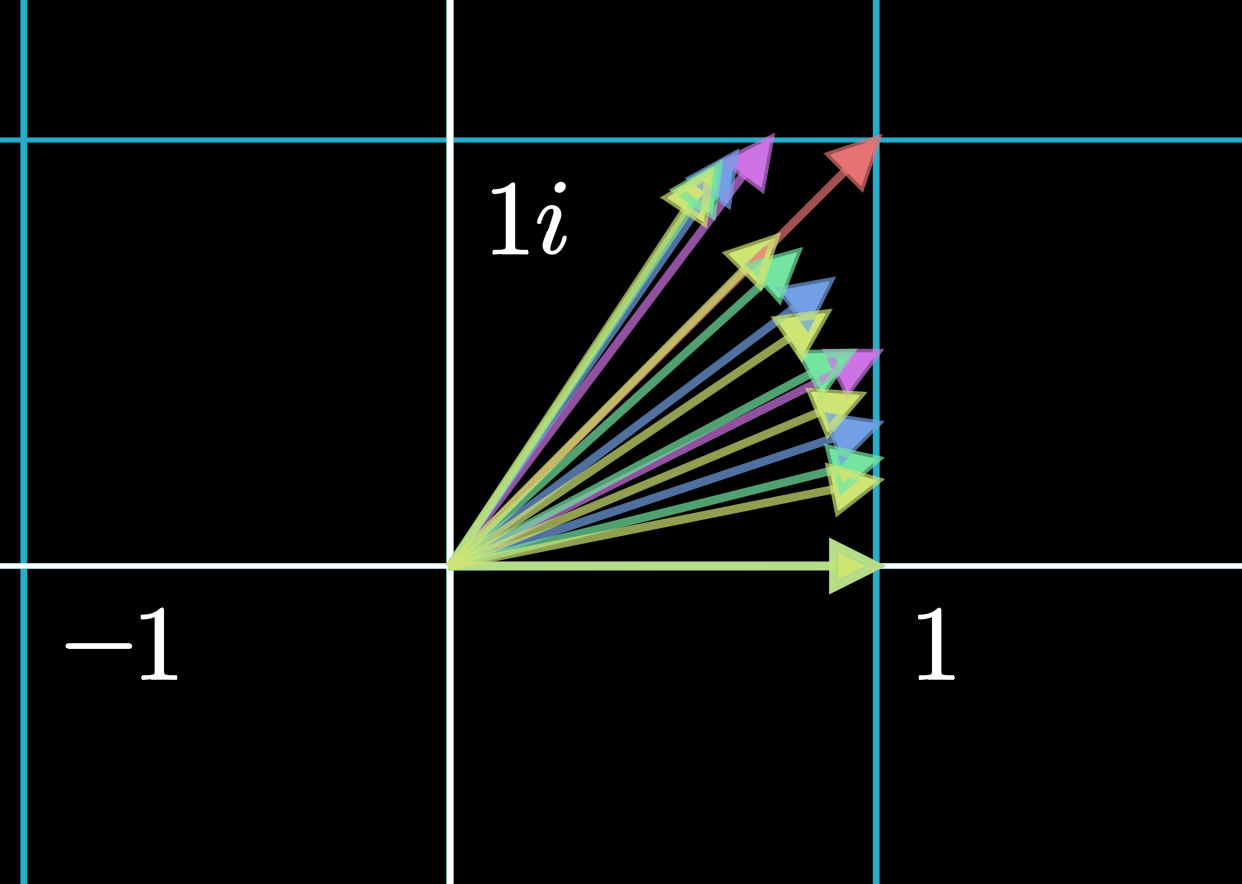
\includegraphics[scale=.4]{onefive} 
\caption{Sequences Generated by n = 1,2,3,4,5 on Argand Diagram}
\end{center}
\end{figure}
\subsection{Is there a geometric interpretation?}
And after seeing this, the most interesting observation seems to be that as n increases,  the vectors it's sequence creates seem to trace out a circular arc. To visualise this hypothesis for larger and larger values of n, its possible to write code to iterate through these drawings. So in the Python library \textit{Manim}, this code can be written:

\begin{lstlisting}
        def intervalValues(z, n):
            output = []
            for f in range(n + 1): # f ranges from 0 to n
                output.append((1 + z / n) ** f) 
            return output # return the sequence of values

        vectors = VGroup() # group of vector objects

        def addVectors(z, n):
            for k in range(1, n + 1): # for each integer up to n
                coords = intervalValues(z, k) # generate it's sequence
                for i in coords: # for every element in the sequence
                    vectors.add( # create a vector from the origin
                        Line(
                            start=ORIGIN,
                            end=complex_to_R3(i),
                            color=rgb_to_color(hsv_to_rgb((n - k + 1) / n,  0.5,  0.9)),  # hue saturation brightness
                        )
                    )
\end{lstlisting}

So drawing the sequences up to a $n = 15$ by calling \texttt{addVectors($i$, 15)}, we get the following visualisation:

\begin{figure}[h]
\begin{center}
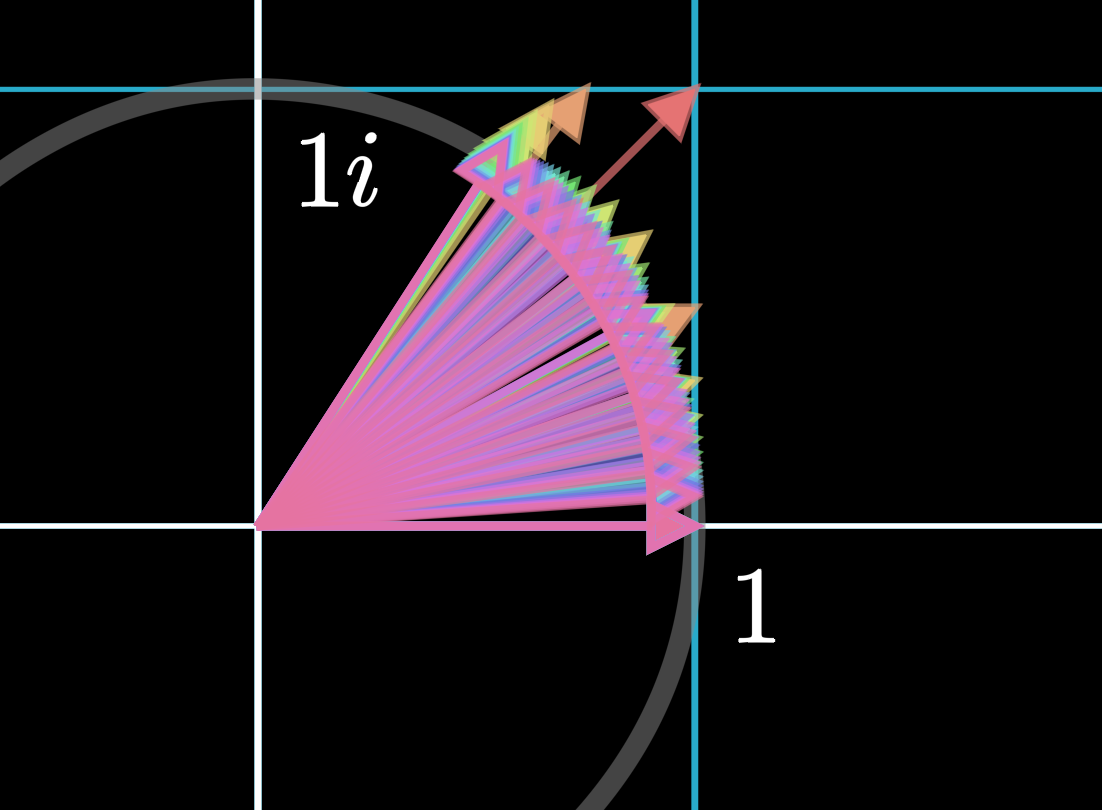
\includegraphics[scale=.37]{onefifteen} 
\caption{Sequences Generated by n = 1-15 on Argand Diagram}
\end{center}
\end{figure}

And even without the encouragingly placed unit circle, it is clear that the pink-most vectors corresponding to the sequence generated by $n=15$ all have a magnitude of roughly one, and draw out an arc of a circle. Most interestingly though, is that these vectors abruptly stop at around $\approx 60$° or 1 radian. So using the same limit definition we can try other \textit{'rates'} of interest to further explore this phenomenon. Considering the sequence with an input of $2i$ instead of $i$:
\begin{align*}
e^{2i} \rightarrow  \left( 1+ \frac{2i}{n} \right) ^0, \left( 1+ \frac{2i}{n} \right) ^1,  ... ,\left( 1+ \frac{2i}{n} \right) ^{n-1},  \left( 1+ \frac{2i}{n} \right) ^{n}
\end{align*}
For $n$ up to 25, we call \textit{addVectors($2i$, 25)}, and get the following:

\begin{figure}[h]
\begin{center}
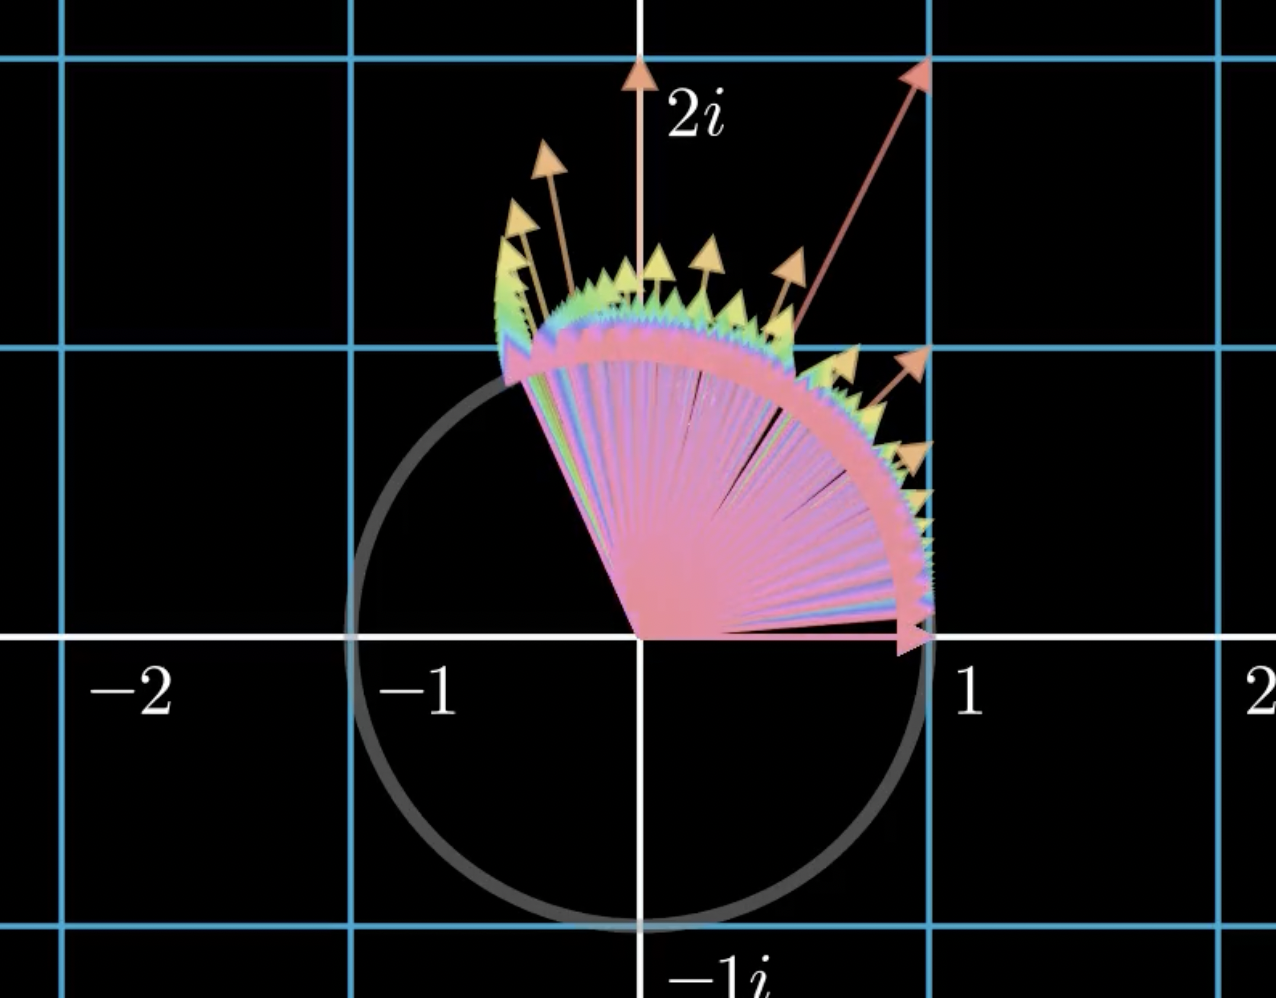
\includegraphics[scale=.5]{twotwentyfive} 
\caption{Sequences for $2i$ Generated by n = 1-25 on Argand Diagram}
\end{center}
\end{figure}

Again here, the pink-most vectors trace out a unit circle and abruptly stop at $\approx 115$° or 2 radians.  This demonstrates the conclusion that the imaginary coefficient determines the angle in radians through which the resultant vector rotates.  (Note that this is another reason $e$ is special, since it is the unique base of complex exponentiation for which this holds true. A base below 2.718... would rotate proportionally less than a radian whereas a base above 2.718... would rotate proportionally more than a radian. Again, this makes intuitive sense because $e^x$ is the unique function where $\frac{d}{dt} e^{rt} = r*e^{rt}$ for an (imaginary) interest rate $r$)
So further testing this hypothesis with the special number $\pi$, as opposed to 1 or 2, we should observe a turn of $\pi$ radians, or half a circle.

\begin{figure}[h]
\begin{center}
\includegraphics[scale=.4]{pisixty} 
\caption{Sequences for $\pi i$ Generated by n = 1-60 on Argand Diagram}
\end{center}
\end{figure}

And by calling \textit{addVectors($\pi i$, 60)}, we get exactly a 1/2 turn about the unit circle, resulting in a vector pointing to $-1$. Or otherwise written:
\begin{align*}
e^{\pi i} = -1
\end{align*}
\subsection{What are the takeaways?}
Another important fact is that since this 'imaginary interest rate' corresponds to a pure rotation along the unit circle of a variable in radians, it seems useful to write this as $e^{\theta i}$. Recalling back to trigonometry,  the x and y coordinates of the unit circle in $\mathbb{R}^2$ define the output of the functions $\cos(\theta )$ and $\sin(\theta)$ respectively, where theta is the angle from the positive x-axis. In our imaginary plane, this y-axis is represented with the imaginary unit. So therefore we can write the more general case:

\begin{align*}
e^{\theta i} = \cos(\theta ) + i\sin(\theta )
\end{align*}

\subsection{So then what's the answer?}
From here I would like to return to my original question: should you take an imaginary interest rate? Well from one of our first formulas, we can calculate the result of an interest rate '$r$' over a time '$t$' with:
\begin{align*}
total = U \left(  1 + \frac{r}{n} \right)  ^{nt}
\end{align*}
And in the limit as $n \to \infty$:
\begin{align*}
total = U*e^{rt}
\end{align*}

But unfortunately, in this continuously compounding case, our newfound knowledge of complex exponentiation tells us that this may not be so fruitful.  Lets say, hypothetically, a bank offers me an interest rate of $i$, and I invest two dollars.  For a few years, my money will be rotating in some intangible dimension where I cannot access it. But, at exactly 3.14159265 years, I get a call from my bank and they tell me I am two dollars in debt, for my money has completed a one half turn about this hypothetical dimension. Annoyed, I refuse to pay the debt, because I know, equipped with my knowledge of complex numbers, that waiting another three-or-so years will net me my initial investment.
\begin{figure}[h]
\begin{center}
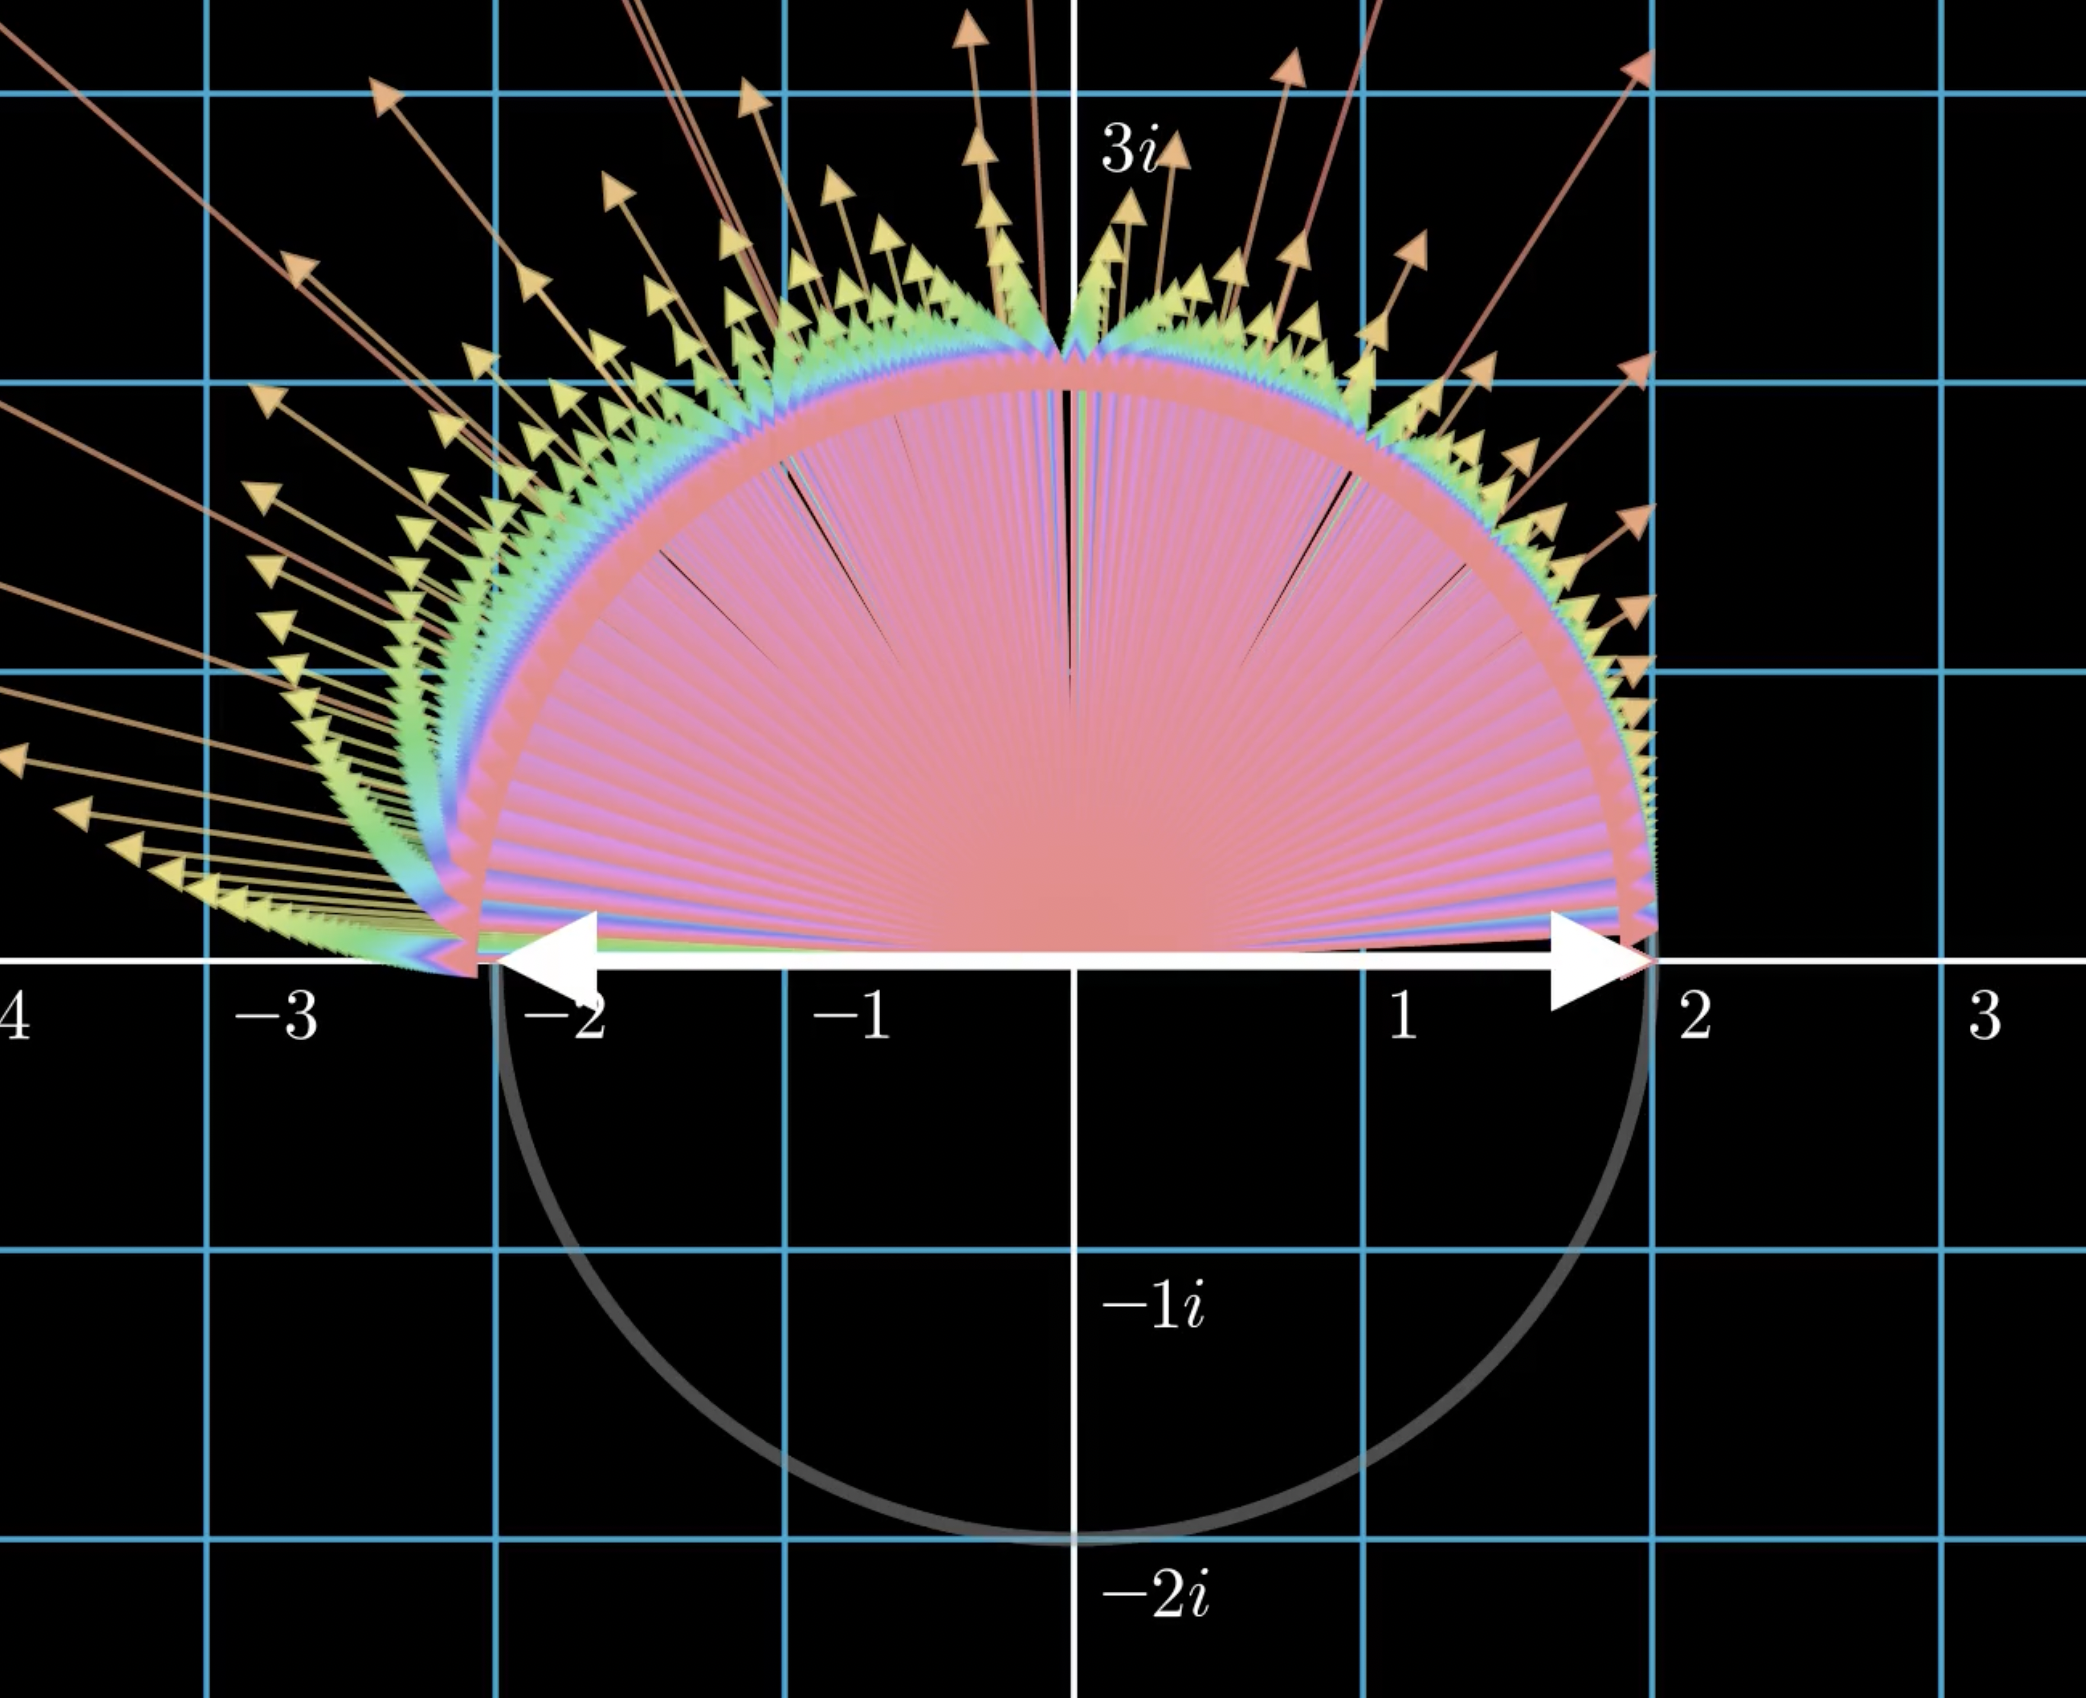
\includegraphics[scale=.3]{pi} 
\caption{My 2\$ After 3.14159 Years}
\end{center}
\end{figure}

Once another 3.14159 years have past, I withdraw my two dollars and reflect on the reliability of this banking establishment.

\begin{figure}[h]
\begin{center}
\includegraphics[scale=.2]{twopi} 
\caption{My 2\$ After 6.28318 Years (with every 10th sequence displayed}
\end{center}
\end{figure}




\section{Conclusion}

Asking questions about findings and applying new algebraic structures to preexisting tools underpins the heart of modern mathematics. For instance, Complex Analysis repeats our process of sticking complex numbers into other ordinary functions and studying their properties. But more broadly, I believe this process of natural understanding and discovery is a crucial way to teach novel concepts. I think this exploration would have succeeded if a reader leaves with a feeling that "if I had a few creative ideas, I definitely could have stumbled upon this mathematical fact." But overall, I think this exploration was enjoyable, especially since the question of imaginary interest rates is a quite a funny/absurd proposition.  (Please don't give the Fed any ideas)\\
Despite its strengths, I would have liked to make a few more connections within this paper. I know the relationship between complex exponentials and trigonometric functions is more fundamental than "it behaves like a circle, so we can use a circle's tools." If I did this paper again, I would have liked to arrive at the power series for $e^x$ either by the binomial expansion from the limit definition, or from the taylor series. This form lends itself better to computer visualisation (in my opinion) and also provides a neat proof of the trigonometric form of complex numbers. Another aspect I would have liked to provide better intuition for is the fact that $e^{it}$ is unique because it rotates at one radian per second. It would have been neat to look at the derivitive of this position vector and how any other base would have the derivative (speed) scaled by a constant. \\
But overall, I enjoyed this exploration and I feel like I came out with a better understanding of complex exponentials. I also enjoyed writing code to aid in visualisation.

\end{document}
